\documentclass[aspectratio=169]{beamer}

% ---- Visual style, aligned with the provided template ----
\usepackage{xcolor}
\definecolor{HermesOrange}{HTML}{F37021}
\definecolor{SoftBlue}{HTML}{EAF3FF}
\definecolor{SoftGreen}{HTML}{EAF7EF}
\definecolor{SoftRed}{HTML}{FFF0EC}
\definecolor{SoftYellow}{HTML}{FFF7D8}
\definecolor{SoftPurple}{HTML}{F0ECFF}
\definecolor{SoftGray}{HTML}{F6F6F6}
\usetheme{Madrid}
\usecolortheme{seahorse}
\setbeamercolor{structure}{fg=HermesOrange}
\setbeamercolor{frametitle}{bg=HermesOrange!10, fg=black!90}
\setbeamercolor{title}{fg=HermesOrange}
\setbeamercolor{block title}{bg=HermesOrange!15, fg=black!90}
\setbeamercolor{block body}{bg=black!2, fg=black!92}
\setbeamercolor{item}{fg=HermesOrange}
\setbeamertemplate{navigation symbols}{}
\setbeamertemplate{itemize item}{\textcolor{HermesOrange}{$\blacktriangleright$}}
\setbeamertemplate{itemize subitem}{\textcolor{HermesOrange}{$\triangleright$}}
\setbeamertemplate{enumerate item}{\textcolor{HermesOrange}{\insertenumlabel.}}

\usepackage{amsmath,amssymb}
\usepackage{array}
\usepackage{booktabs}
\usepackage{tikz}
\usetikzlibrary{arrows.meta,positioning,calc,fit}
\newcommand{\paper}[1]{\textcolor{HermesOrange!90!black}{\textbf{#1}}}
\newcommand{\stlG}{\mathbf{G}}
\newcommand{\stlF}{\mathbf{F}}
\newcolumntype{L}[1]{>{\raggedright\arraybackslash}p{#1}}

\title[NL, STL, and Safe RL]{From Natural Language to Safe Reinforcement Learning with STL}
\subtitle{NL2TL (2023) \texorpdfstring{$\to$}{->} UAV STL Repair (2026) \texorpdfstring{$\to$}{->} Safe RL via Shielding (2017)}
\author{Yuhang Zhang}
\institute{EECS, Washington State University}
\date{\today}

\begin{document}

% ===== 1 =====
\begin{frame}
\titlepage
\end{frame}

% ===== 2 =====
\begin{frame}{The Shared Story}
\begin{center}
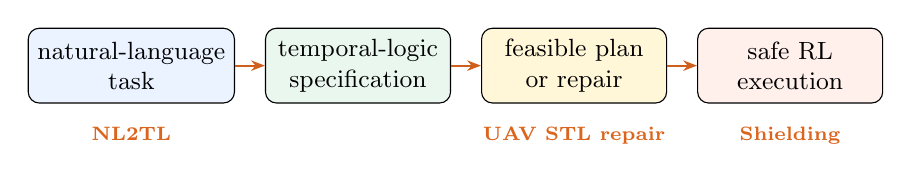
\begin{tikzpicture}[
  box/.style={draw,rounded corners,align=center,font=\small,minimum width=2.35cm,minimum height=0.95cm},
  arr/.style={-{Stealth[length=5pt]},thick,HermesOrange!85!black}
]
  \node[box,fill=SoftBlue] (nl) {natural-language\\task};
  \node[box,fill=SoftGreen,right=0.38cm of nl] (stl) {temporal-logic\\specification};
  \node[box,fill=SoftYellow,right=0.38cm of stl] (plan) {feasible plan\\or repair};
  \node[box,fill=SoftRed,right=0.38cm of plan] (rl) {safe RL\\execution};
  \draw[arr] (nl)--(stl);
  \draw[arr] (stl)--(plan);
  \draw[arr] (plan)--(rl);
  \node[font=\scriptsize,align=center,below=0.18cm of nl] {\paper{NL2TL}};
  \node[font=\scriptsize,align=center,below=0.18cm of plan] {\paper{UAV STL repair}};
  \node[font=\scriptsize,align=center,below=0.18cm of rl] {\paper{Shielding}};
\end{tikzpicture}
\end{center}

\vspace{0.5em}
\begin{block}{Reading logic}
\small
The three papers cover adjacent but different parts of the same route. NL2TL learns how language becomes temporal logic. The UAV paper checks whether an STL task can produce a feasible trajectory. Shielding enforces a given temporal-logic safety rule during RL.
\end{block}

\vspace{0.2em}
\small
The missing interface is: \textbf{natural-language safety requirements should become executable safety constraints for RL}, not only a translated formula or a one-shot planned trajectory.
\end{frame}

% ===== 3 =====
\begin{frame}{Paper 1: NL2TL Learns the Logic Skeleton}
\begin{columns}[T]
\column{0.52\textwidth}
\begin{block}{Problem}
\small
Translate natural-language instructions into temporal logic across domains, despite limited manually labeled NL--TL data.
\end{block}

\begin{block}{Core idea}
\small
\begin{itemize}
  \item Hide domain objects and actions as atomic propositions: \texttt{prop\_1}, \texttt{prop\_2}, \ldots
  \item Fine-tune T5 on lifted NL--STL pairs, so the model mainly learns temporal operators and formula structure.
  \item Use GPT-3 to help synthesize data and, in application, detect atomic propositions in the original sentence.
\end{itemize}
\end{block}

\column{0.44\textwidth}
\begin{block}{Example}
\small
\[
\begin{array}{c}
\text{``Eventually visit A and always avoid B.''}\\[0.3em]
\Downarrow\\[0.3em]
\stlF\, \texttt{prop\_1}\ \wedge\ \stlG\, \neg\texttt{prop\_2}
\end{array}
\]
\vspace{-0.3em}
\small
Then \texttt{prop\_1} and \texttt{prop\_2} are filled with domain-specific predicates such as regions, objects, or events.
\end{block}

\begin{block}{Reported signal}
\footnotesize
T5-large reaches about \(97.5\%\) exact match on lifted data; full NL-to-STL with GPT-3 AP detection is around \(95\%\)--\(97\%\) across tested domains.
\end{block}
\end{columns}
\end{frame}

% ===== 4 =====
\begin{frame}{NL2TL: What It Gives and What It Does Not}
\begin{columns}[T]
\column{0.48\textwidth}
\begin{block}{Advantages}
\small
\begin{itemize}
  \item Separates logical structure from domain grounding.
  \item Reduces the need for large domain-specific labeled datasets.
  \item Shows that a fine-tuned sequence model can outperform few-shot GPT-3/GPT-4 end-to-end translation.
  \item Gives a practical recipe: AP detection plus lifted formula generation.
\end{itemize}
\end{block}

\column{0.48\textwidth}
\begin{block}{Limitations for safety control}
\small
\begin{itemize}
  \item Exact formula match is not the same as trajectory-level safety.
  \item Atomic proposition grounding still depends on domain conventions and language ambiguity.
  \item The generated formula is not checked for dynamic feasibility.
  \item There is no RL policy, safety monitor, or runtime intervention mechanism.
\end{itemize}
\end{block}
\end{columns}

\vspace{0.35em}
\begin{center}
\small
NL2TL is best viewed as the \textbf{language-to-specification front end}, not as a complete safety-control system.
\end{center}
\end{frame}

% ===== 5 =====
\begin{frame}{Paper 2: UAV NL-to-STL with MILP Repair}
\begin{center}
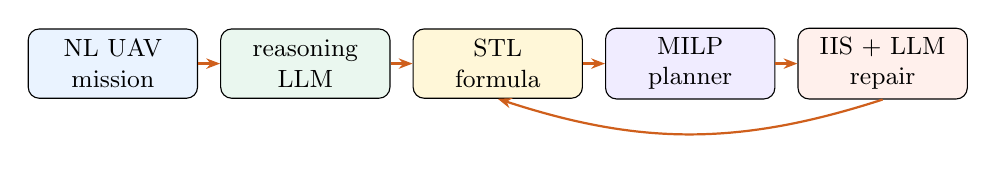
\begin{tikzpicture}[
  box/.style={draw,rounded corners,align=center,font=\small,minimum width=2.15cm,minimum height=0.88cm},
  arr/.style={-{Stealth[length=5pt]},thick,HermesOrange!85!black}
]
  \node[box,fill=SoftBlue] (nl) {NL UAV\\mission};
  \node[box,fill=SoftGreen,right=0.28cm of nl] (llm) {reasoning\\LLM};
  \node[box,fill=SoftYellow,right=0.28cm of llm] (stl) {STL\\formula};
  \node[box,fill=SoftPurple,right=0.28cm of stl] (milp) {MILP\\planner};
  \node[box,fill=SoftRed,right=0.28cm of milp] (repair) {IIS + LLM\\repair};
  \draw[arr] (nl)--(llm);
  \draw[arr] (llm)--(stl);
  \draw[arr] (stl)--(milp);
  \draw[arr] (milp)--(repair);
  \draw[arr] (repair.south) to[bend left=18] (stl.south);
\end{tikzpicture}
\end{center}

\vspace{0.4em}
\begin{block}{Key move}
\small
The paper does not stop after translation. It encodes STL satisfaction and UAV dynamics into a mixed-integer linear program. If the problem is infeasible, an IIS diagnosis identifies conflicting STL parts; the LLM chooses whether to relax time or predicate requirements, while safety constraints are never relaxed.
\end{block}

\begin{block}{Repair example}
\small
\[
\stlG_{[0,T]}\neg R_o \wedge \stlF_{[0,20]}R_g
\quad\leadsto\quad
\stlG_{[0,T]}\neg R_o \wedge \stlF_{[0,30]}R_g .
\]
The obstacle-avoidance rule stays hard; only the goal-reaching deadline is relaxed.
\end{block}
\end{frame}

% ===== 6 =====
\begin{frame}{UAV STL Repair: What It Adds and What It Still Assumes}
\begin{columns}[T]
\column{0.48\textwidth}
\begin{block}{Advantages}
\small
\begin{itemize}
  \item Connects language translation to executable motion planning.
  \item Uses formal MILP feasibility rather than only text-level correctness.
  \item Keeps safety constraints non-negotiable during repair.
  \item Demonstrates the idea in simulation and real low-altitude UAV experiments.
\end{itemize}
\end{block}

\column{0.48\textwidth}
\begin{block}{Limitations for our direction}
\small
\begin{itemize}
  \item The downstream executor is a model-based finite-horizon planner, not an RL learner.
  \item The method assumes known dynamics, known map regions, and MILP-encodable constraints.
  \item It repairs one planned trajectory, not learning-time exploration over many episodes.
  \item Safety/task separation and numeric grounding must already be meaningful.
\end{itemize}
\end{block}
\end{columns}

\vspace{0.35em}
\begin{center}
\small
This is the closest paper to the language--STL side, but it answers a planning question rather than a safe-RL question.
\end{center}
\end{frame}

% ===== 7 =====
\begin{frame}{Paper 3: Shielding Makes RL Respect a Given Safety Rule}
\begin{columns}[T]
\column{0.52\textwidth}
\begin{block}{Problem}
\footnotesize
RL can learn high-reward behavior while violating safety constraints during training or execution. Reward penalties alone do not provide formal safety guarantees.
\end{block}

\begin{block}{Core idea}
\footnotesize
Given a temporal-logic safety specification \(\varphi_s\) and a conservative finite-state abstraction of the environment, synthesize a shield that sits between the agent and the environment.
\end{block}

\column{0.44\textwidth}
\begin{center}
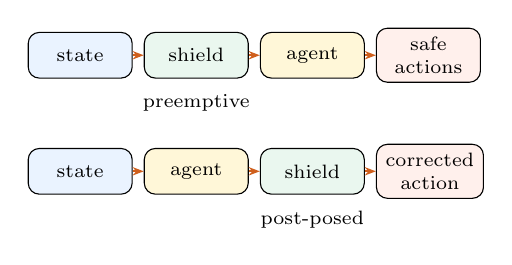
\begin{tikzpicture}[
  box/.style={draw,rounded corners,align=center,font=\scriptsize,minimum width=1.32cm,minimum height=0.58cm},
  arr/.style={-{Stealth[length=4pt]},thick,HermesOrange!85!black}
]
  \node[box,fill=SoftBlue] (env1) {state};
  \node[box,fill=SoftGreen,right=0.14cm of env1] (sh1) {shield};
  \node[box,fill=SoftYellow,right=0.14cm of sh1] (ag1) {agent};
  \node[box,fill=SoftRed,right=0.14cm of ag1] (act1) {safe\\actions};
  \draw[arr] (env1)--(sh1);
  \draw[arr] (sh1)--(ag1);
  \draw[arr] (ag1)--(act1);
  \node[font=\scriptsize,below=0.08cm of sh1] {preemptive};

  \node[box,fill=SoftBlue,below=0.88cm of env1] (env2) {state};
  \node[box,fill=SoftYellow,right=0.14cm of env2] (ag2) {agent};
  \node[box,fill=SoftGreen,right=0.14cm of ag2] (sh2) {shield};
  \node[box,fill=SoftRed,right=0.14cm of sh2] (act2) {corrected\\action};
  \draw[arr] (env2)--(ag2);
  \draw[arr] (ag2)--(sh2);
  \draw[arr] (sh2)--(act2);
  \node[font=\scriptsize,below=0.08cm of sh2] {post-posed};
\end{tikzpicture}
\end{center}
\end{columns}

\vspace{0.05em}
\begin{center}
\footnotesize
Guarantee target: \textbf{correctness} and \textbf{minimum interference}; the shield blocks only actions that could force a future violation.
\end{center}
\end{frame}

% ===== 8 =====
\begin{frame}{Shielded RL: What It Gives and What It Does Not}
\begin{columns}[T]
\column{0.48\textwidth}
\begin{block}{Advantages}
\small
\begin{itemize}
  \item Safety is enforced at runtime, including during learning.
  \item The shield is mostly independent of the internal RL algorithm.
  \item It reasons ahead: an action can be blocked before the violation becomes immediate.
  \item It separates safety correctness from reward optimization.
\end{itemize}
\end{block}

\column{0.48\textwidth}
\begin{block}{Limitations for language-driven safety}
\small
\begin{itemize}
  \item The safety specification \(\varphi_s\) is assumed to be given by an expert.
  \item A conservative environment abstraction is required.
  \item Rich numeric STL constraints need grounding and abstraction before shielding.
  \item It does not translate, repair, or disambiguate natural-language requirements.
\end{itemize}
\end{block}
\end{columns}

\vspace{0.35em}
\begin{center}
\small
Shielding is the strongest safety-execution piece, but it starts after the specification already exists.
\end{center}
\end{frame}

% ===== 9 =====
\begin{frame}{Natural Gap: NL Safety Constraints for RL}
\begin{block}{Focused problem}
\footnotesize
Input: an RL environment \(M\) and a language task \(L=(L_{\mathrm{goal}},L_{\mathrm{safe}})\). Translate \(L_{\mathrm{safe}}\) into grounded STL and test whether it makes RL measurably safer:
{\scriptsize
\[
\max_{\pi}\ \mathbb{E}_{\pi}\!\left[\sum_{t=0}^{H}\gamma^t r_t\right]
\quad
\text{s.t.}\quad
\Pr_{\tau\sim\pi}\!\left[\tau \models \varphi_{\mathrm{safe}}\right]\ge 1-\delta .
\]
}
\end{block}

\vspace{-0.35em}
\begin{columns}[T]
\column{0.5\textwidth}
\begin{block}{Why this is not exactly prior work}
\scriptsize
\begin{itemize}
  \item NL2TL translates formulas, but does not enforce them.
  \item UAV repair enforces STL through MILP planning, not RL learning.
  \item Shielding enforces RL safety, but assumes a formal rule.
\end{itemize}
\end{block}

\column{0.46\textwidth}
\begin{block}{Key difficulties}
\scriptsize
\begin{itemize}
  \item Ground vague language into predicates and time windows.
  \item Separate hard safety from soft task preference.
  \item Evaluate trajectory violations, not only exact match.
  \item Handle infeasibility and abstraction error.
\end{itemize}
\end{block}
\end{columns}
\end{frame}

\end{document}
